\documentclass{article}

\usepackage[margin=1in]{geometry} 
\usepackage[english]{babel}
\usepackage[T1]{fontenc}
\usepackage[utf8]{inputenc}
\usepackage{amsmath,amsthm,amssymb,amsfonts, fancyhdr, color, comment, graphicx, environ}
\usepackage{xcolor}
\usepackage{mdframed}
\usepackage[shortlabels]{enumitem}
\usepackage{indentfirst}
\usepackage{hyperref}
\usepackage{lastpage}
\usepackage{listingsutf8}
%\usepackage{ff++listings}
\usepackage{amsmath}
\DeclareMathOperator{\Tr}{Tr}

\usepackage{physics}
\usepackage{amsfonts}
\usepackage{float}
\PassOptionsToPackage{hyphens}{url}\usepackage{hyperref}

\newenvironment*{remerciements}{%
\renewcommand*{\abstractname}{Acknowledgements}
\begin{abstract}
}{\end{abstract}}

\usepackage{xurl}

\renewcommand{\footrulewidth}{0.8pt}
\hypersetup{
    colorlinks=true,
    linkcolor=blue,
    filecolor=magenta,      
    urlcolor=blue,
}

\pagestyle{fancy}

\newenvironment{problem}[2][Etape]
    { \begin{mdframed}[backgroundcolor=gray!20] \textbf{#1 #2} \\}
    {  \end{mdframed}}

\newenvironment{solution}{\textbf{Réponse}}

\lhead{Florent Pollet}
\rhead{ES2A EEP-02} 
\chead{\textbf{Vaccine strategies}}
\lfoot{Véronique Stoven}
\cfoot{Mines Paris}
\rfoot{\thepage/\pageref*{LastPage}}


\let\up\textsuperscript

\usepackage{biblatex}
\addbibresource{biblio/biblio.bib}

%\usepackage[backend=bibtex]{biblatex}
\usepackage[nottoc, notlof, notlot]{tocbibind}

% lack of references IN the text?

\begin{document}

    \title{\Large ES2A EEP-02  \\[0.5cm]
        \bf\Large Vaccine strategies}
\author{\large Florent Pollet \ \\}
\date{\large\today}

\makeatletter
    \begin{titlepage}
        \begin{center}
	   { 
\includegraphics[width=12cm]{imgs/mp_logo.png}}
	   {\ \\ \ \\}
        \vbox{}\vspace{2cm}
            {\@title }\\[1cm] 
            %{ \includegraphics[width=7cm]{imgs/cover.PNG}}\\[1cm]
            {\@author}

            {\large \ \\ Supervisor: \bf Véronique Stoven\\ \ \\}
            {\@date\\}

        \end{center}

        \vspace{4cm}
        \begin{figure}[H]
            \centering
            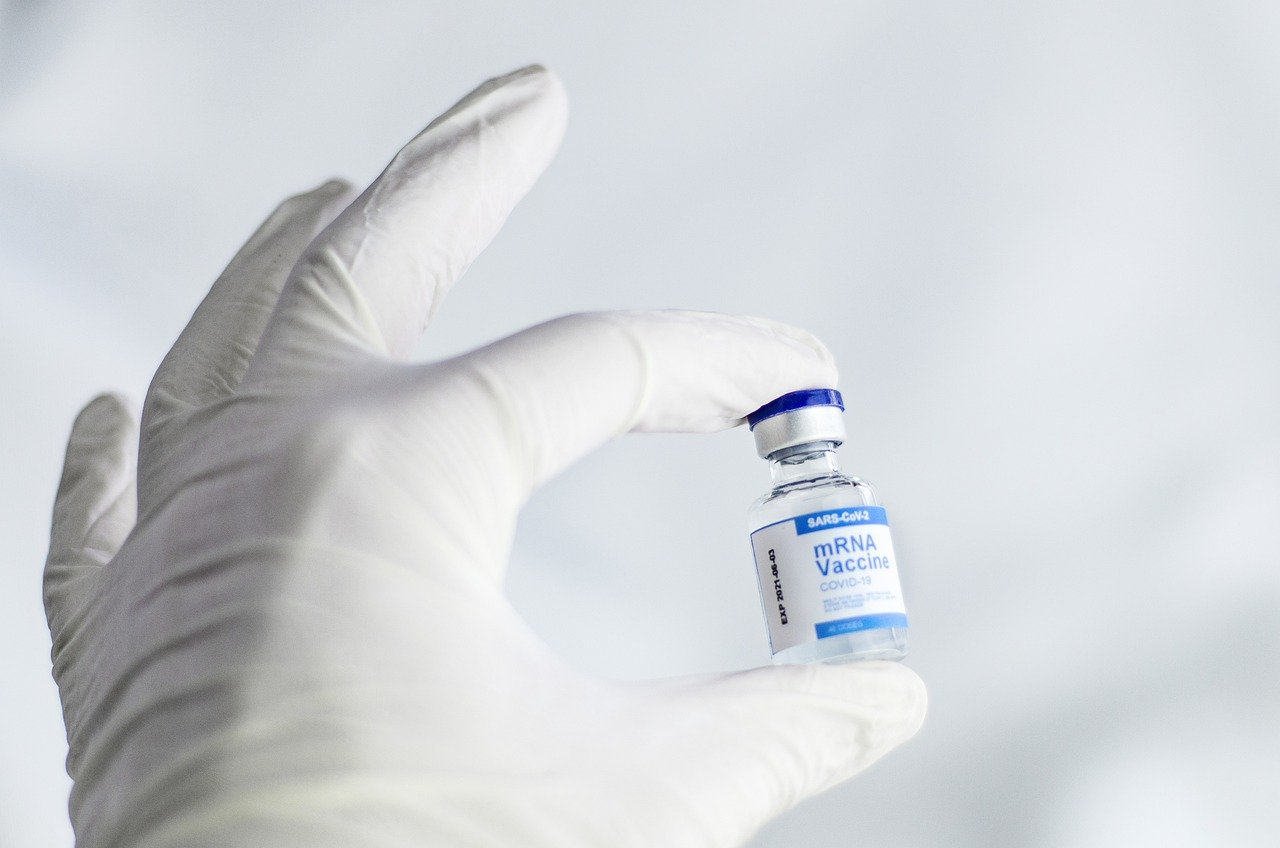
\includegraphics[width=0.4\textwidth]{imgs/vaccineCover.jpg}
        \end{figure}

    \end{titlepage}


    \begin{abstract}        
        In a context of a pandemic and major doubts towards vaccination among populations, this paper deals with vaccine strategies, especially how mRNA vaccines are revolutionizing them.
        It is clear that immunology represents a complex field of science,
            and nowadays the breakthroughs in biotechnologies are offering new possibilities to accelerate vaccine development, efficiency and safety as well as a better understanding
            our immune system.
        This paper aims at summarizing the different vaccine techniques with a special attention to mRNA vaccines\footnote{Messenger RiboNucleic Acid}, in order to
            have an overview of the current vaccine strategies which are going to evolve.
        % implications, finding, methods ? go further ?
    \end{abstract}

        
    \begin{remerciements}
        I cannot express enough thanks to my teacher Véronique Stoven for her interesting lessons about molecular and synthetic biology,
            which inspired me this topic.
        I absolutely loved doing research and writing this report.
    \end{remerciements}


    \tableofcontents


    \newpage

    \makeatother

    \section{Introduction}

    Vaccines represent an amazing invention which saved millions of lives in the world since 2000 \autocite{HowManyLives2021}.
    Even if vaccination is not new, the recent pandemic of COVID-19 brought to the forefront this field, generating great advances but also important debates about safety, ethics and politics.
    It is necessary to take into account all these changes and to adapt to avoid a backward step and the rejection of these opportunities. 
    
    Therefore it would be interesting to better understand the recent evolutions in vaccine strategies and technologies as well as the consequences it may have on society.
    
    Firstly, I will briefly recall the history of vaccination, detailing the different types of vaccines which have been developed.
    Secondly, I will present the technology of mRNA (messenger ribonucleic acid) vaccines which currently constitute major advances.
    Thirdly, I will observe how society is integrating these developments and what issues remain to be solved.

    \section{A brief history of vaccines}

        \subsection{Discovery of the principle}

            The principle of vaccination could come from or be related to the idea of mithridatism,
             that is to say the ability to gain protection against a poison by taking several benign amounts.
            
            Variolization, which corresponds to injecting smallpox pustules to gain immunity against smallpox, began in China around the 10\up{th} century \autocite{canouiHistoryPrinciplesVaccination2019}. 
            Before the nineteenth century, several persons realized variolization in England. However, in 1798, this is Jenner who made a link between cowpox and smallpox: 
                cowpox could be an attenuated version of smallpox.            
                Besides, The word "vaccination" comes from the Latin word "vacca", which means "cow".

            The idea of vaccination is to create an individual, long-term and efficient protection against a pathogen (like a virus or a bacteria), without causing serious symptoms.
            This is made possible thanks to the memory of the human immune system: it can learn to react quickly and efficiently against another infections.
            It constitutes a deferred but durable protection. To better understand the principle, some basic knowledge in the immune system is needed.

            \subsubsection*{The immune system at a glance}

                In the medical field, the immune system is mainly composed of two parts:

                \begin{itemize}
                    \item The innate immune system. After the infection, it is the first system to react. It is mainly represented by Natural Killers (NK) cells,
                            phagocytes and dentritric cells which play an important role to initiate the adaptive response\footnote{The details for each different type 
                                of cells will not be covered in this report.}.
                    \item The adaptive (or acquired) immune system. This one is subdivised into two categories: 
                        \begin{itemize}
                            \item The cellular response, thanks to lymphocytes T (thymus) CD8+ (cluster of designation). They are cytotoxic and they can kill the infected cells.
                                    To be efficient, in most cases, they need the major histocompatibility complex, 
                                    that is to say cells which are presenting molecules from the virus in a special manner.
                            \item The humoral response, thanks to lymphocytes B (Bursa of Fabricius). They produce antibodies (immunoglobulines, abbreviated Ig),
                                    which are proteins able to 
                                    neutralize microbial effectors, from bacteria and viruses. 
                                    A schematic structure is delivered in \ref{fig:antigens}.
                                    Antibodies need antigens of the pathogens, which are proteins expressed by the pathogen, to recognize it.
                        \end{itemize}

                        \begin{figure}
                            \centering
                            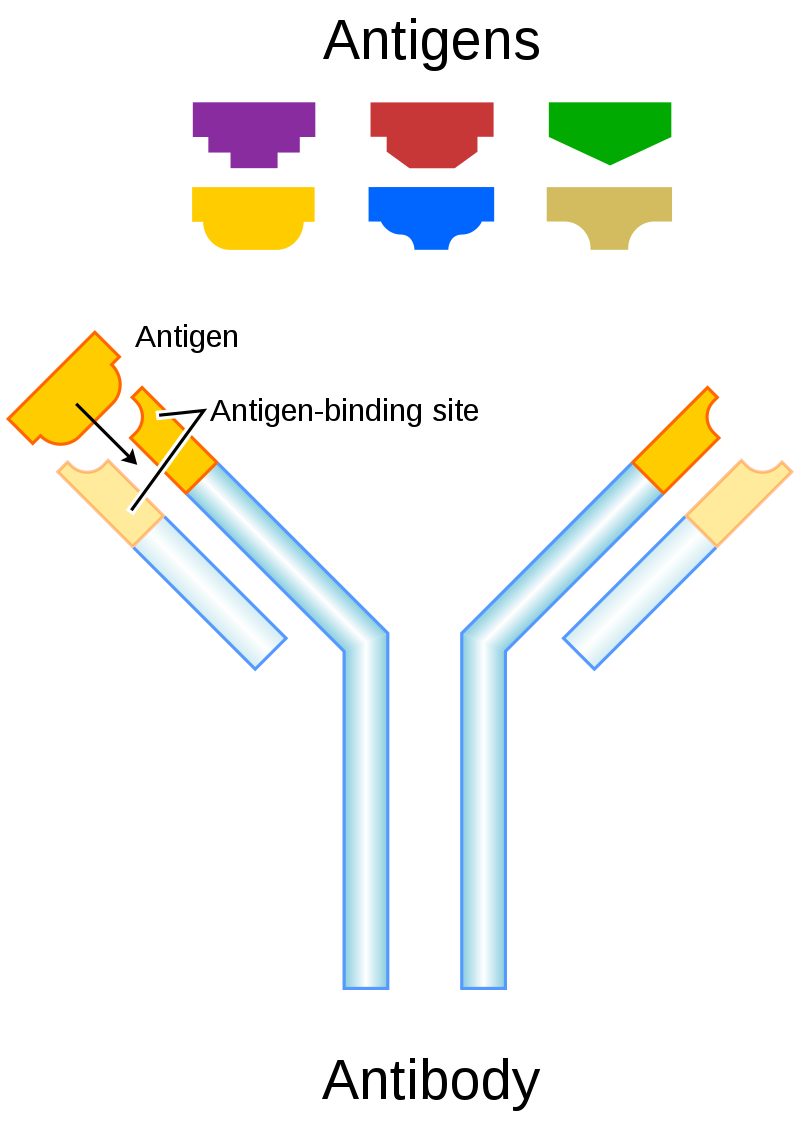
\includegraphics[width=0.3\textwidth]{imgs/Antigen.png}
                            \caption{Schematic diagram of an antibody and antigens (source \emph{Wikipedia})}
                            \label{fig:antigens}
                        \end{figure}

                        Lymphocytes T CD4+ (helpers) regulate both responses.
                        The specifity of the adaptive immune system is its memory thanks to specific T and B memory cells, 
                            and the phenomenon can be easily observed using the concentration of immunoglobulines in the blood.
                        
                            \begin{figure}
                                \centering
                                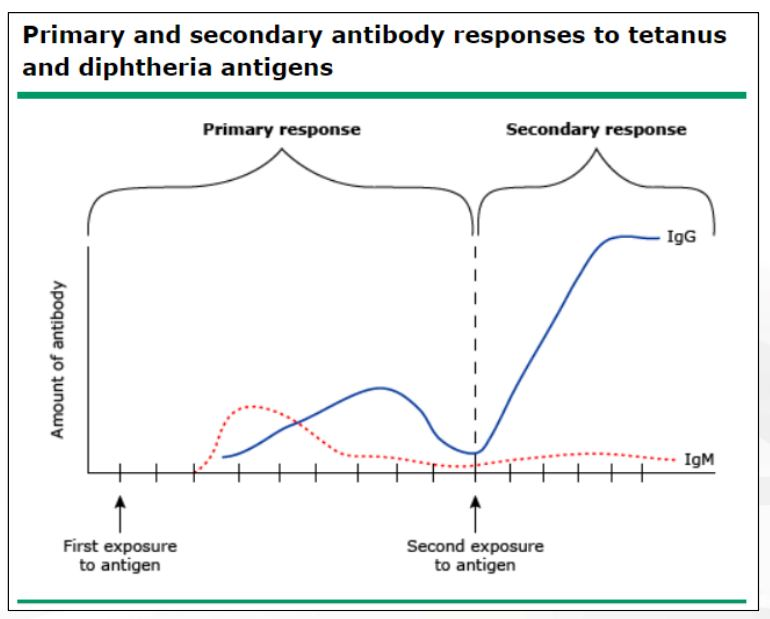
\includegraphics[width=0.7\textwidth]{imgs/PrimarySecondaryResponses.JPG}
                                \caption{Primary and secondary responses to specific antigens \autocite{pinkComparisonImmunityGeneral}}
                                \label{fig:responses}
                            \end{figure}

                        The graph \ref{fig:responses} shows that the response after the first infection is less important and slower than after the second one.
                        It also compares the concentration of IgM, an immoglobuline which is non-specific, 
                            versus IgG, which is more specific towards microbial effectors such as toxines or proteins:
                            it proves that the adaptive immune system becomes efficient after the innate system, and that there is a memory effect on the second infection.                     

                        The cellular response is more complicated to quantify.

                        As regards pathogens, the incubation period can be short (pneumococcus) or long (hepatitis B virus).

                        It is important to notice that the immune system is very different according to the age of the person: the main phenomenon when ageing is immunosenescence,
                            which makes the immune system less reactive and dynamic.
                \end{itemize}
              
        \subsection{First generation of vaccines}
            
            It is only between 1870 and 1885 with Pasteur's works (helped by Emile Roux and Emile Duclaux), 
                that the first vaccines were developed \autocite{plotkinHistoryVaccination2014}.
            The first official vaccines that he conceived were against chicken cholera, anthrax, swine erysipelas and then rabies.

            The first generation of vaccines consists in pathogens which are live and weakened (attenuated) or killed (inactivated). Live weakened vaccines are the most immunogenic,
                but they should be prepared carefully. Despite being efficient, there are still high risks using them if virus are not attenuated enough:
                one can develop the disease and transmit it to another immunocompromised person. Otherwise, vaccines can be killed for example with heat/chemical treatments, and they
                are less dangerous, however there is a need for adjuvants (from the Latin word "adjurvare", which means "to help") 
                to make them immunogenic, and the response can be more humoral than cellular.

            Adjuvants can be very diverse and numerous as well as their mechanism of action: killed mycobacteria, oils, 
                aluminium salts, microparticles, squalanes, ligands of 
                PRRs (Pattern Recognition Receptor)... 
                They aim at amplifying the reaction for each individual (especially old people whose immune system is less dynamic) and 
                at reducing the quantity of active substance needed (dose sparing). The dosage should be very cautious not to hide the active substance.
                
            To prepare those vaccines, cell culture is often needed, which can be a long and complex process.
            To weaken viruses, other environments than human cells are used such as chicken cells so that the virus is no more adapted to human cells...
            The virus or the bacteria is therefore replicated in adverse conditions several times. Main vaccines of this type are BCG
            (Bacillus Calmette-Guérin vaccine, against tuberculosis) or the Mumps vaccine. 

            It is important to note that different vaccines can be combined together,
            like with the MMRV vaccine (Mumps, Measles, Rubella and Varicella: a tetravalent vaccine).
            It is not dangerous for health and it avoids too many injections for children,
            who have to develop an immunity for many diseases in the first years.
            
            A classical example for killed vaccines could be the polio vaccine.  
                       
            %https://www.pnas.org/content/111/34/12283

            Thanks to the development of immunology and microbiology, in particular the ability to isolate pathogens, vaccines were better understood
                and it led to the development of a new type of vaccines.

            The method of production of these vaccines also evolved over time. With genetic engineering and reverse genetics, that is to say,  
                contrary to forward genetic, the ability to know which phenotypes can be controlled by different genetic sequences,
                it allows a better treatment of viruses to select inactivated vaccines.

        \subsection{Second generation of vaccines}

            % https://vaccine-safety-training.org/subunit-vaccines.html

            This generation demands more development and technological advances,
                to use subunits of viruses such as protein antigens or inactivated toxins from the pathogen. %recombinant protein components (antigens for instance).
            There is also the need for adjuvant, which are substances which trigger a powerful immune response; otherwise the vaccine would not be effective. 
            The response is mainly humoral: sometimes it cannot activate Toll-Like Receptors on dentritic cells needed for a complete response.

            Subunits vaccines (also called acellular vaccines) are stable and safe, with no risk to induce the disease but the right part of the virus should be choosen.
                They can be protein-based, with polysaccharides, which is a sugar capsule produced by some pathogens (however it has less effect than proteins), or both (it is then called conjugate).
            Inactivated toxins are called anatoxins. These are toxins which have lost their toxic power thanks to heat and formaldehyde, but not totally their immunogenic ability.

            To produce these units, the pathogen is cultivated at a large scale before using chemicals to destroy and separate the parts of the pathogen.

            Lots of recent vaccines use this technique: influenza, hepatitis A, HPV (Human papillomavirus infection), pertussis, tetanus (anatoxin). 
                The first approved subunit vaccine was against hepatitis B in 1981 in the United States. 
                At that time, it was a breakthrough because it represented the first vaccine to also protect against liver cancer and against a sexually transmitted disease.

            With the development of medecine, with a principle close to vaccination,
                serotherapy also appeared, which means solely injecting immunoglobulines, but it is only humoral, passive and temporary.

        \subsection{Towards a third generation}

            The third generation of vaccines can be described as genetic vaccines, since it is using genetic sequences to support the information of the pathogen. 
            It was made possible thanks to the latest discoveries in biotechnologies and genetics such as gene sequencing \autocite{chavdaDNAVaccinesSARSCoV22021}.  

            There are three main categories:
            \begin{itemize}
                \item Viral vector vaccines: a specific gene of the pathogen is put into an innocuous virus for humans. 
                        This harmless virus can deliver the selected genetic material of the pathogen into the human cells.
                        Then the cells produce proteins from the pathogen which can be used to train the immune system as a classic vaccine.
                        For instance, the vaccines from the firm AstraZeneca and the Oxford University or Janssen against Covid-19 rely on this technique.
                        A major drawback of viral vector vaccines is that it also makes us immune against the vector virus, 
                            which in the future will have difficulties to deliver the genetic material.
                \item mRNA vaccines: this will be discussed in the next section.
                \item pDNA (Plasmid DesoxyriboNucleic Acid) vaccines: the gene from the pathogen is encoded with DNA instead of RNA
                    and it is injected in our cells thanks to the same technique as mRNA vaccines.
                    Nevertheless it must be carefully studied because of the possible effects on human DNA such as DNA integration.
            \end{itemize}

            It is useful to note that the majority of vaccines requires intramuscular injection, instead of subcutaneous, intradermic, or intravenous (or even mucosa).
                Indeed muscle tissue contains the best dentritic cells, which trigger the adaptive immune response.
            There may be several doses and boosters to maximize efficiency and send reminders for the immune system. 

            % tab récapulatif

    \section{mRNA vaccines: a promising technology}

        \subsection{Principle}

                First and firemost, it is important to understand the differences between the terms \emph{in vitro}, \emph{in vivo} and \emph{in situ} (from the Latin).
                \begin{itemize}
                    \item \emph{in vitro} which means "in glass" refers to tube experiments.
                    \item \emph{in vivo} which means "within the living" refers to experiments on living organisms (humans, animals, plants...).
                    \item \emph{in situ} which means "on site" refers to the usual place an event should happen (for example at a specific point in the human body).
                \end{itemize}
                The aim with this new type of vaccine is to realize a minimum of steps \emph{in vitro} and \emph{in vivo} while preparing the vaccine and
                    let people's cells do most of the "job", giving them only information about a part of the pathogen instead of the whole microbe thanks
                    to mRNA \autocite{maruggiMRNATransformativeTechnology2019}.         
                It is worth noting that \emph{in vitro} traduction to get the protein is still difficult, and alternative methods should be used for the other
                    types of vaccines, which make them more complex to produce and it requires more time.

                The two major incentives which were met were quicker development (with financial and medical interests) and a wider and safer immune response.
                It can even lead to other uses and it creates new perspectives as regards therapies.

                Therefore, mRNA represents the blueprint for a protein of the pathogen, it does not need a virus as a vector
                    and it has fewer risks/unknown effects than pDNA, even if it is a very fragile molecule.
                The way to convey mRNA relies on nano-lipids instead of viruses, which can efficiently enter the cells.


        \subsection{Development}

            The first tests were realized in the 1990s by Wolff \autocite{wolffDirectGeneTransfer1990}.
            But much progress has been needed in the 2000s as regards the synthesis of mRNA.

            The main steps to develop a mRNA vaccine, summarized in \ref{fig:mRNAvac}, are:
            \begin{itemize}
                \item First, scientists have to find an antigen that can characterize the pathogen thanks to reverse genetics.
                \item Second, the gene encoding this antigen is sequenced. 
                    The sequence can be shared on the Internet all over the world, allowing global research and speeding up development.
                \item Then, the gene can be synthetized thanks to recent biotechnologies like artificial gene synthesis, often called DNA printing. 
                    Firms like Thermo Fisher Scientific are offering a lot of services in this field.
                % https://www.thermofisher.com/fr/fr/home/references/ambion-tech-support/probe-labeling-systems/general-articles/the-basics-in-vitro-transcription.html
                \item This DNA constitutes a DNA template plasmid, and it is traduced \emph{in vitro} into mRNA.
                        All this process is realized thanks to enzymes, especially the RNA polymerase. The DNase then degrades the template DNA.
                        It is also an enzyme which adds the required 5' cap, stabilizing the molecule.
                \item A step of purification is then critical to obtain an efficient mRNA vaccine. 
                        Current techniques are for instance high-performance liquid chromatography (HPLC) or fast protein liquid chromatography (FPLC).
                        Enzymes, remaining DNA and incorrect RNA transcripts are removed.
                        There are also double-stranded RNA (dsRNA) which can alter the immune activation if they are still present.
                        Finally some tests (such as potency tests) are conducted to check the product.
            \end{itemize} % test d'activité =/= safety test

            In current vaccines, the nucleotide U is replaced by 1-methyl-3'-pseudouridylyl, noted $\Psi$, as indicated in \ref{fig:mRNAvac_detail}.
            Empirically it increases the efficiency of the vaccine, it is a kind of fine tuning.
            The synthesis is deployed at a large scale to produce the millions of doses which are needed.

            % https://www.iconsci.com/what-are-the-differences-between-fplc-and-hplc/
                        
            \begin{figure}
                \centering
                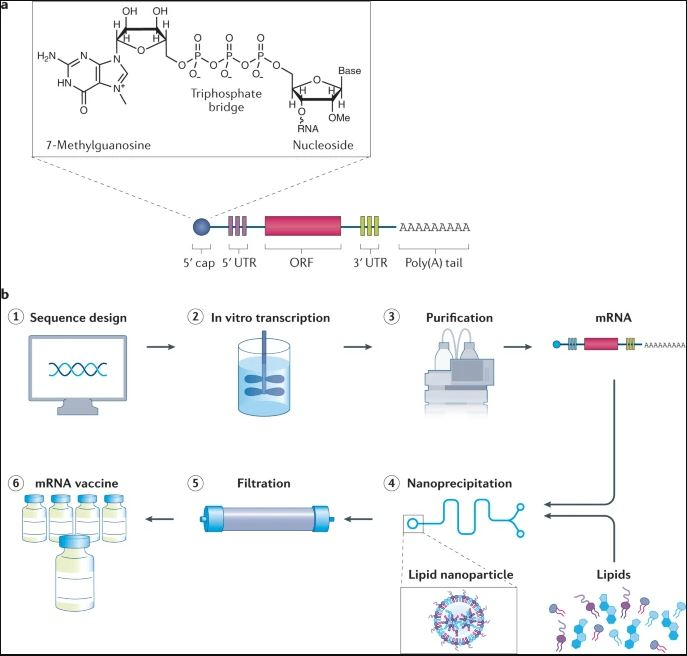
\includegraphics[width=0.75\textwidth]{imgs/mRNA_Vaccine.JPG}
                \caption{Preparation of an mRNA vaccine \autocite{MRNAVaccinesInfectious}}
                \label{fig:mRNAvac}
            \end{figure}
            
            \begin{figure}
                \centering
                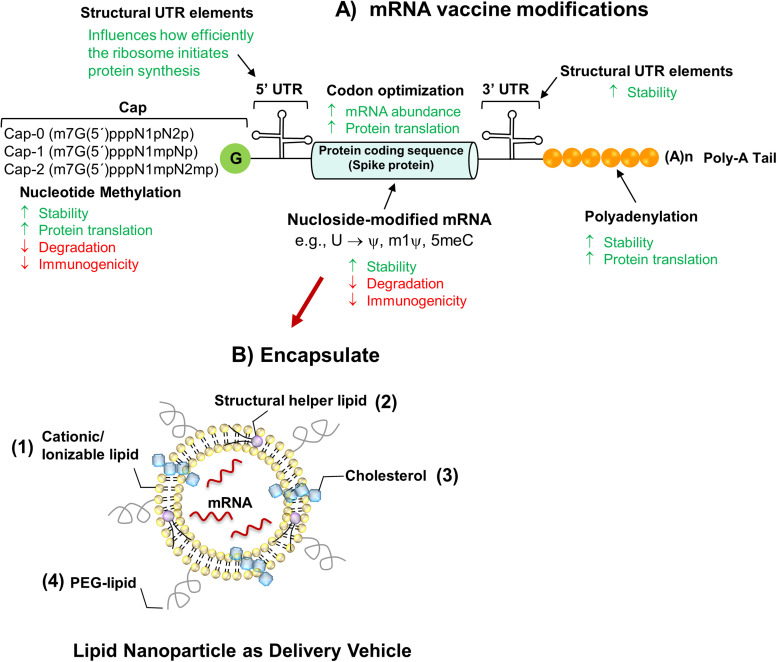
\includegraphics[width=0.65\textwidth]{imgs/RNA2.jpg}
                \caption{mRNA structure \autocite{granados-riveronEngineeringCurrentNucleosidemodified2021}}
                \label{fig:mRNAvac_detail}
            \end{figure}

            Nowadays, there are two major types of mRNA vaccines, as the Figure \ref{fig:mRNAtypesnext} shows:
            \begin{itemize}
                \item Conventional mRNA which only corresponds to the studied gene.
                \item Self-amplifying mRNA which also encodes the replication machinery to produce many antigens.
            \end{itemize}
            
            \begin{figure}
                \centering
                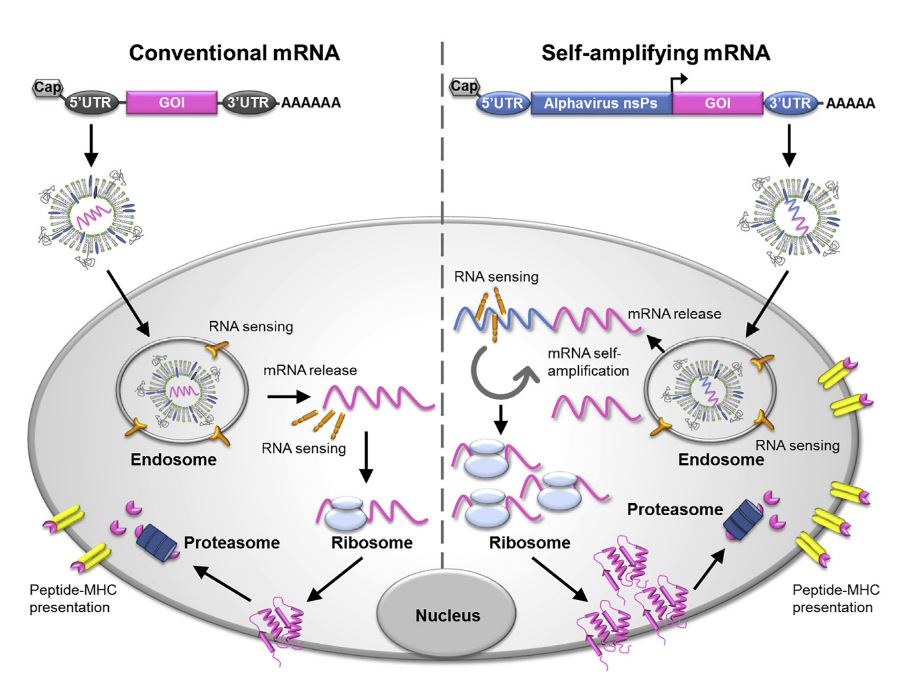
\includegraphics[width=0.65\textwidth]{imgs/mRNA_action.JPG}
                \caption{mRNA vaccine's operating mode \autocite{MRNATransformativeTechnology}}
                \label{fig:mRNAtypesnext}
            \end{figure}

        % Code source of the modified Spike-encoding gene : https://zestedesavoir.com/billets/3750/explorons-le-code-source-du-vaccin-biontech-pfizer-contre-le-sars-cov-2/

        % Severe acute respiratory syndrome coronavirus 2 (SARS‑CoV‑2)
        % https://www.medpagetoday.com/special-reports/exclusives/91604
        % Upon vaccination, nucleic acid-based vaccines mimic a viral infection to express vaccine antigens in situ, resulting in induction of both humoral and cytotoxic T cell responses.
        % https://www.sciencedirect.com/science/article/pii/S1525001619300413?via%3Dihub
     
        \subsection{A breakthrough technology}

            Among the technologies of the third generation, it is the most promising compared to viral vectors and pDNA vaccines in terms of efficiency and safety.
            It merges all recent discoveries as explained in \ref{fig:revolution}.
            
            \begin{figure}
                \centering
                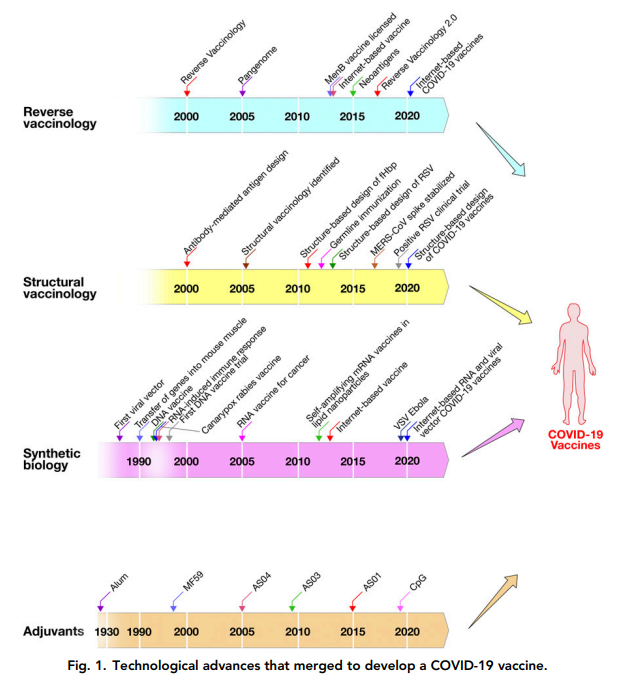
\includegraphics[width=0.75\textwidth]{imgs/Revolution.PNG}
                \caption{Technical advances for genetic vaccines \autocite{rappuoliVaccinologyPostCOVID192021}}
                \label{fig:revolution}
            \end{figure}

            Moreover, several assets can be observed:
            \begin{itemize}
                \item It embodies the idea of "vaccine on demand". It would allow people to face epidemics like for Zika and Ebola as well as pandemics.
                    In some classical vaccines, mRNA traduction can be achieved \emph{in vitro} to produce the pathogen proteins to inject, but it is a long and complicated process.
                    The Figure \ref{fig:devVaccine} shows how it has been possible to develop a vaccine so quickly:
                        \begin{itemize}
                            \item The disease is very common to have volunteers and data.
                            \item There was no need of major cell cultures and protein production.
                            \item Regulations and authorities were very responsive to analyze results and interact with pharmaceutical companies.
                        \end{itemize}
                \item It creates a complete immune response (humoral and cellular), without needing adjuvants like other vaccines:
                    they have intrinsic adjuvant properties since they can be recognized by PRRs
                    (as shown on \ref{fig:mRNAtypesnext}, proteins are expressed at the surface of the cell), initiating an innate response activating
                    the subsequent adaptive immune system (thanks to dendritic cells and cytokines for instance).
            \end{itemize}

            \begin{figure}
                \centering
                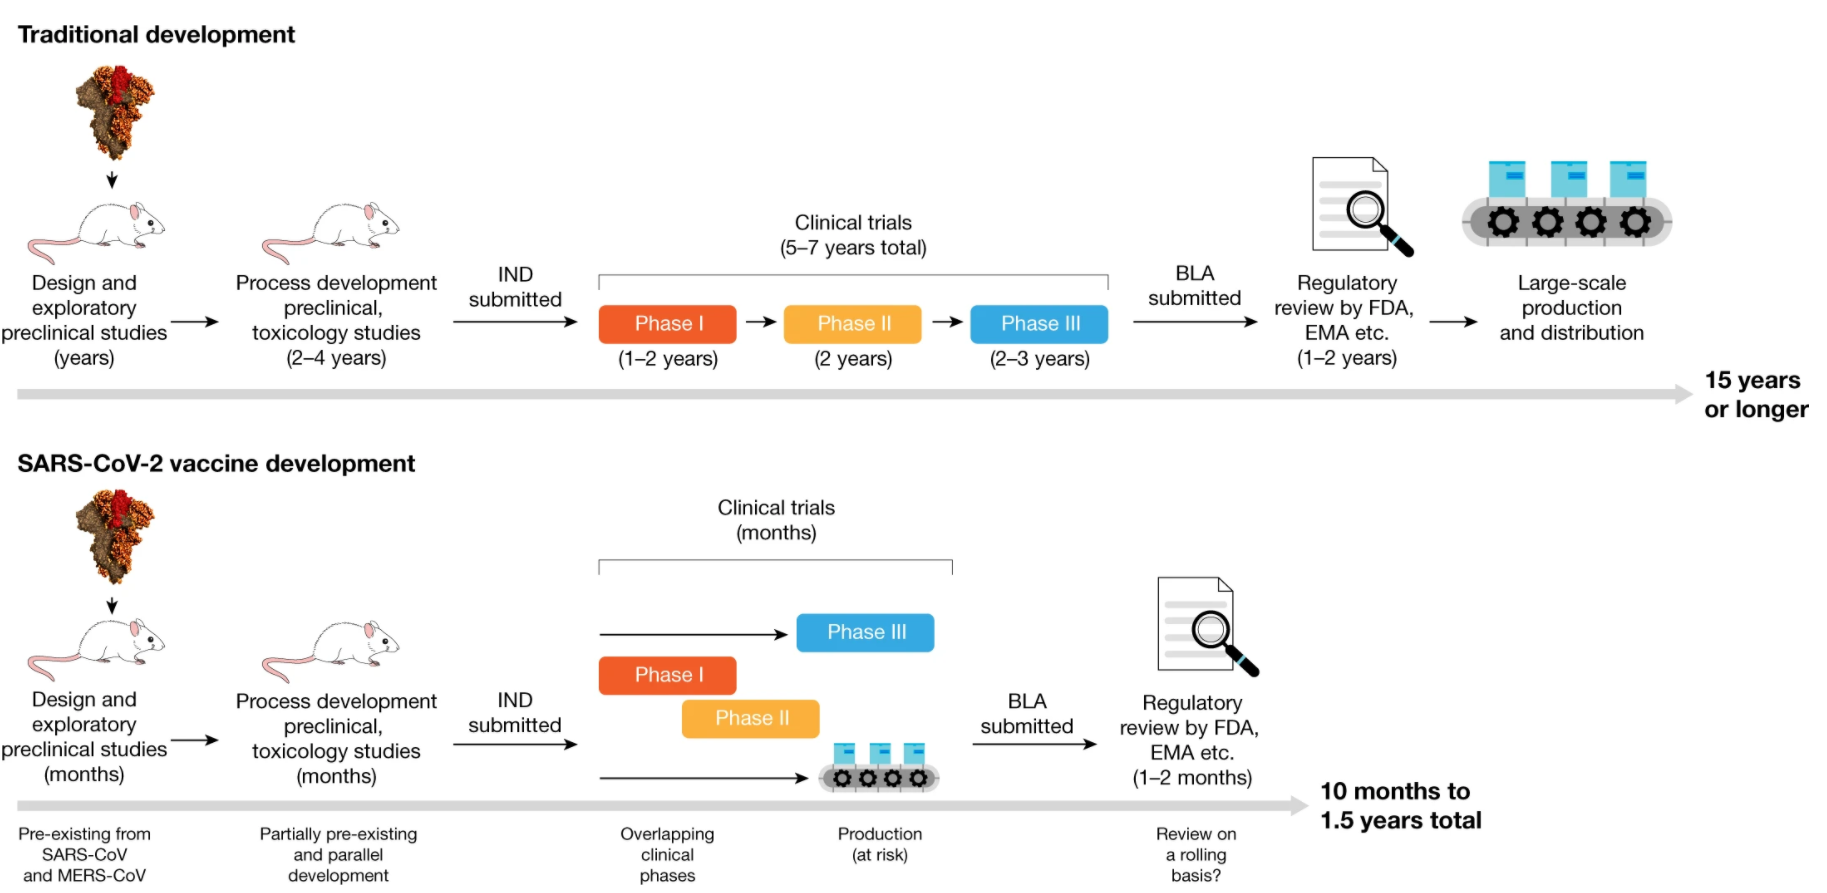
\includegraphics[width=0.9\textwidth]{imgs/CovidDev.png}
                \caption{Comparison of vaccine developments \autocite{krammerSARSCoV2VaccinesDevelopment2020}}
                \label{fig:devVaccine}
            \end{figure}

            Nonetheless, some problems are still faced these days:
            \begin{itemize}
                \item It is very difficult to preserve the vaccine because mRNA is not stable. 
                    Preservation should be at a temperature around -70°C...
                \item The duration of expression is short because mRNA is quickly degraded, 
                    so vaccines may need several doses.
                \item The risk of anaphylatic shock, which is a severe and life-threatening allergic reaction, is quite high and difficult to predict, even if it is very rare.
                        Some Guillain–Barré syndromes, which correspond to a serious side effect, were also declared.
            \end{itemize}
            The classical side effects of vaccines, namely local pain, fever and fatigue during a few days are still present
                 (and it indicates that people's immune system is reacting).
            
            Currently scientists are trying to improve the efficiency of mRNA vaccines by trying different caps,
            doing codon optimization (using DNA as an intermediary may change some codons used by the virus when it is RNA; there is also the codon usage bias),
            adding complementary RNAs or dsRNA... \autocite{MRNATransformativeTechnology}

        % https://www.amazon.fr/Basic-Immunology-Book-Functions-Disorders-ebook/dp/B07N8ZKYPQ?asin=B07N8ZKYPQ&revisionId=4497585a&format=1&depth=1

    \section{New stakes for vaccines in the 21\up{st} century}

        \subsection{World inequalities}

            It is crucial that these new techniques should not increase distribution inequalities in the world.
            Countries in Africa already have difficulties to organize vaccination campaigns and some diseases are still widespread (like polio) compared to other countries.
            COVID-19 is another example of these inequalities, as \ref{fig:world_ineq} shows. It is all the more difficult to deliver them
                with the transport and storage constraints of these fragile mRNA vaccines.
            
                \begin{figure}
                    \centering
                    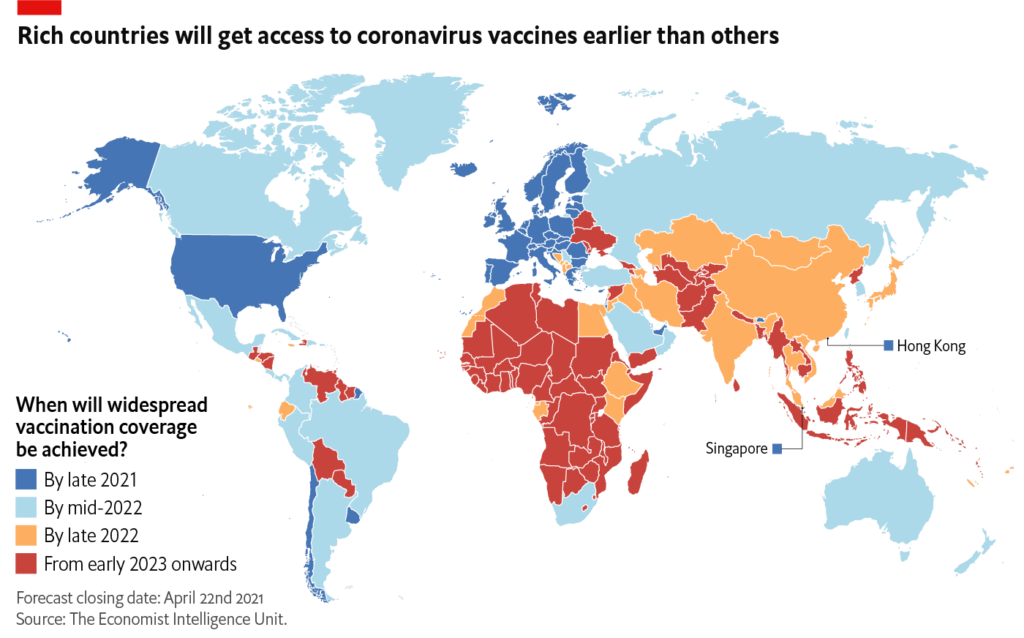
\includegraphics[width=0.8\textwidth]{imgs/Inequalities.png}
                    \caption{COVID-19 vaccine deliveries (source \emph{The Economist})}
                    \label{fig:world_ineq}
                \end{figure}

            Economic models for pharmaceutical firms should be revised and unified for a better global health.
            International organizations such as the World Health Organization (WHO) try to coordinate and help every state develop vaccine agenda.
            For instance, the WHO prepared the "immunization agenda 2030", which is a global strategy (the Global Vaccine Action Plan) 
                to help fight the most serious diseases in countries with difficulties,
                asking rich nations to put efforts together.

        % https://www.immunizationagenda2030.org/scorecard for slides and explanations

        \subsection{Public policies}
 
            Vaccination is a major lever for public health, as the Figure \ref{fig:numberofcases} proves.
            When the vaccine coverage is high, that is to say the percentage of the population who is vaccinated, thus immuzined against a pathogen, 
                the number of cases of the disease collapses.
            Therefore it means less pain for people and fewer patients in hospitals.

            Three types of population are distinguished:
            \begin{itemize}
                \item The general population, which has no particular risk or exposure.
                \item The population at-risk, composed of immunodeficient people, elderly and people with comorbidities.
                \item The exposed population, made up of professional working in endemic zones.
            \end{itemize}          

            \begin{figure}
                \centering
                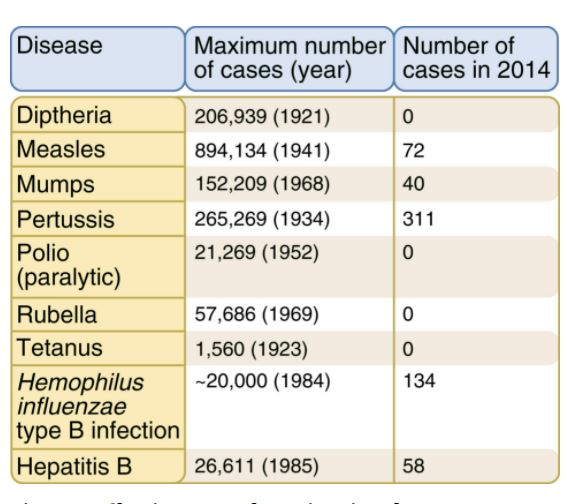
\includegraphics[width=0.5\textwidth]{imgs/NumberOfCases.JPG}
                \caption{Vaccine positive effects \autocite{HowManyLives2021}} % source fausse probablement, à revoir
                \label{fig:numberofcases}
            \end{figure}

            As a consequence, the France authorities decided to enforce a vaccine agenda, shown in \ref{fig:vacAgenda}, with many vaccines
                which can be combined (multivalent vaccine) to avoid too many injections if there are no interferences between them.
            Nonetheless, the obligation for the smallpox vaccine was removed in the 80s because the disease disappeared from the region
                thanks to a high and durable vaccine coverage.
            Other vaccines are necessary when travelling to regions with other diseases, for example yellow fever in Africa.

            Due to immunosenescence, which is the aging of the immune system which becomes less reactive, five vaccines are recommended
                for people over 60 years old: anti-influenza, anti-tetanus, anti-diphtheria, anti-pertussis and anti-pneumococcal.

            \begin{figure}
                \centering
                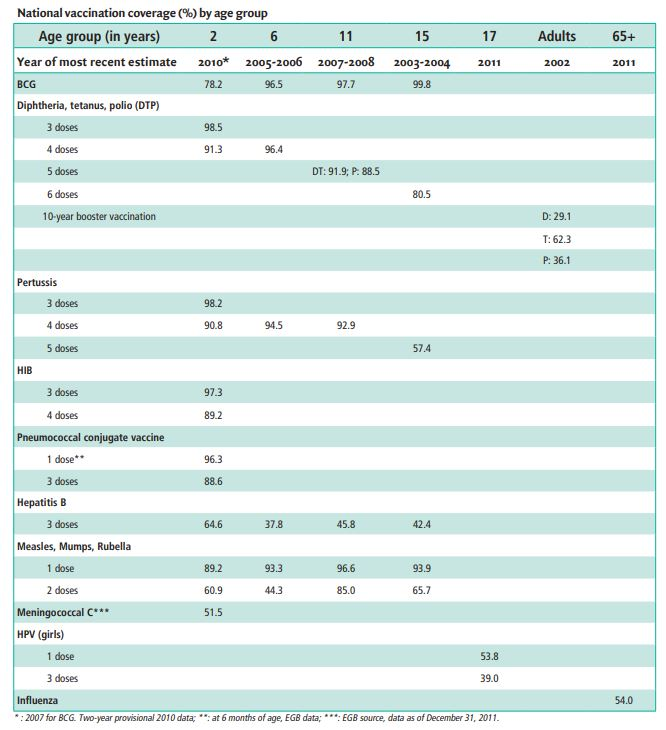
\includegraphics[width=0.7\textwidth]{imgs/VaccineSchedule.JPG}
                \caption{Vaccine schedule in France (Institut de veille sanitaire, InVS) \autocite{spfAssessmentVaccinationCoverage}}
                \label{fig:vacAgenda}
            \end{figure}

            Moreover, regulations are established to assure quality in this critical field.
                Good manufacturing practice (abbreviated GMP) represents a minimum standard for medecine manufacturers,
                concerning mRNA production at an industrial level for instance. In the United States, the Food and Drug Administration (FDA) is determining it, and in Europe
                it is the European Medicines Agency (EMA).

            Despite all these efforts of governments, public acceptancy is lukewarm, as a recent survey shown in \ref{fig:survey} reveals.
            The paradox is that the countries with fewer vaccination campaigns are the most confident in vaccines and those with the best campaigns are quite doubtful.          
                    
                \begin{figure}
                    \centering
                    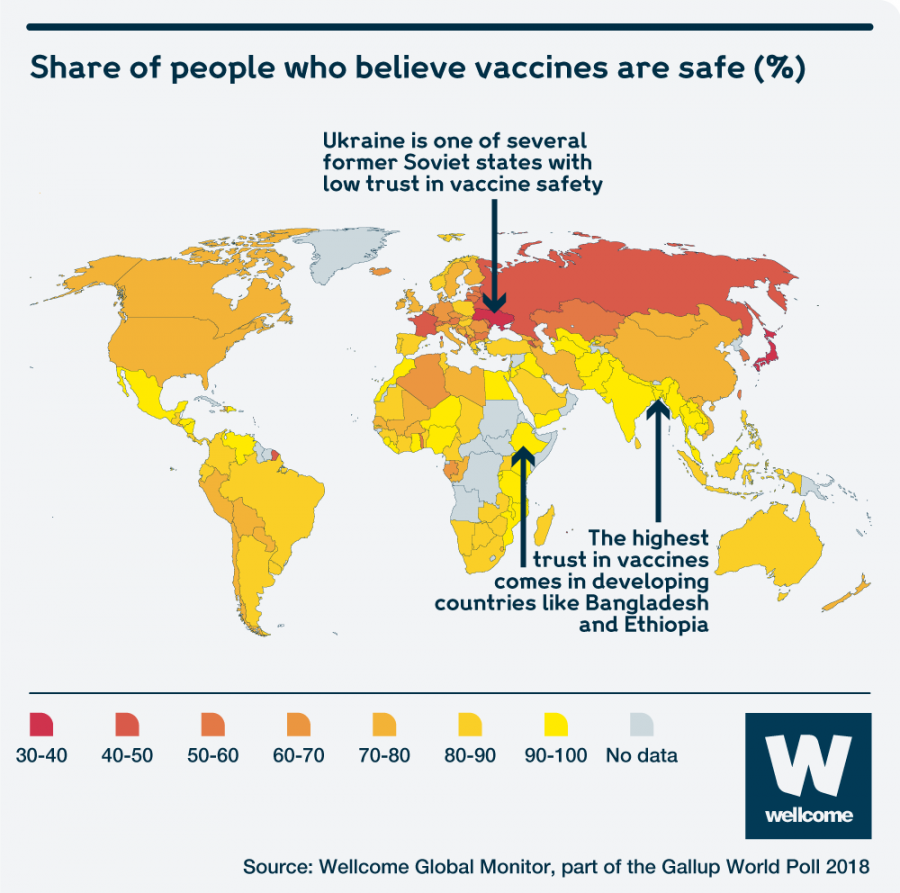
\includegraphics[width=0.5\textwidth]{imgs/VaccineHesitancy.png}
                    \caption{Global survey about vaccine safety \autocite{SurveyRevealsEuropean}}
                    \label{fig:survey}
                \end{figure}

            This can be partially explained because people only see side effects and do not observe the benefits anymore as \ref{fig:perception} explains.
        
            \begin{figure}
                    \centering
                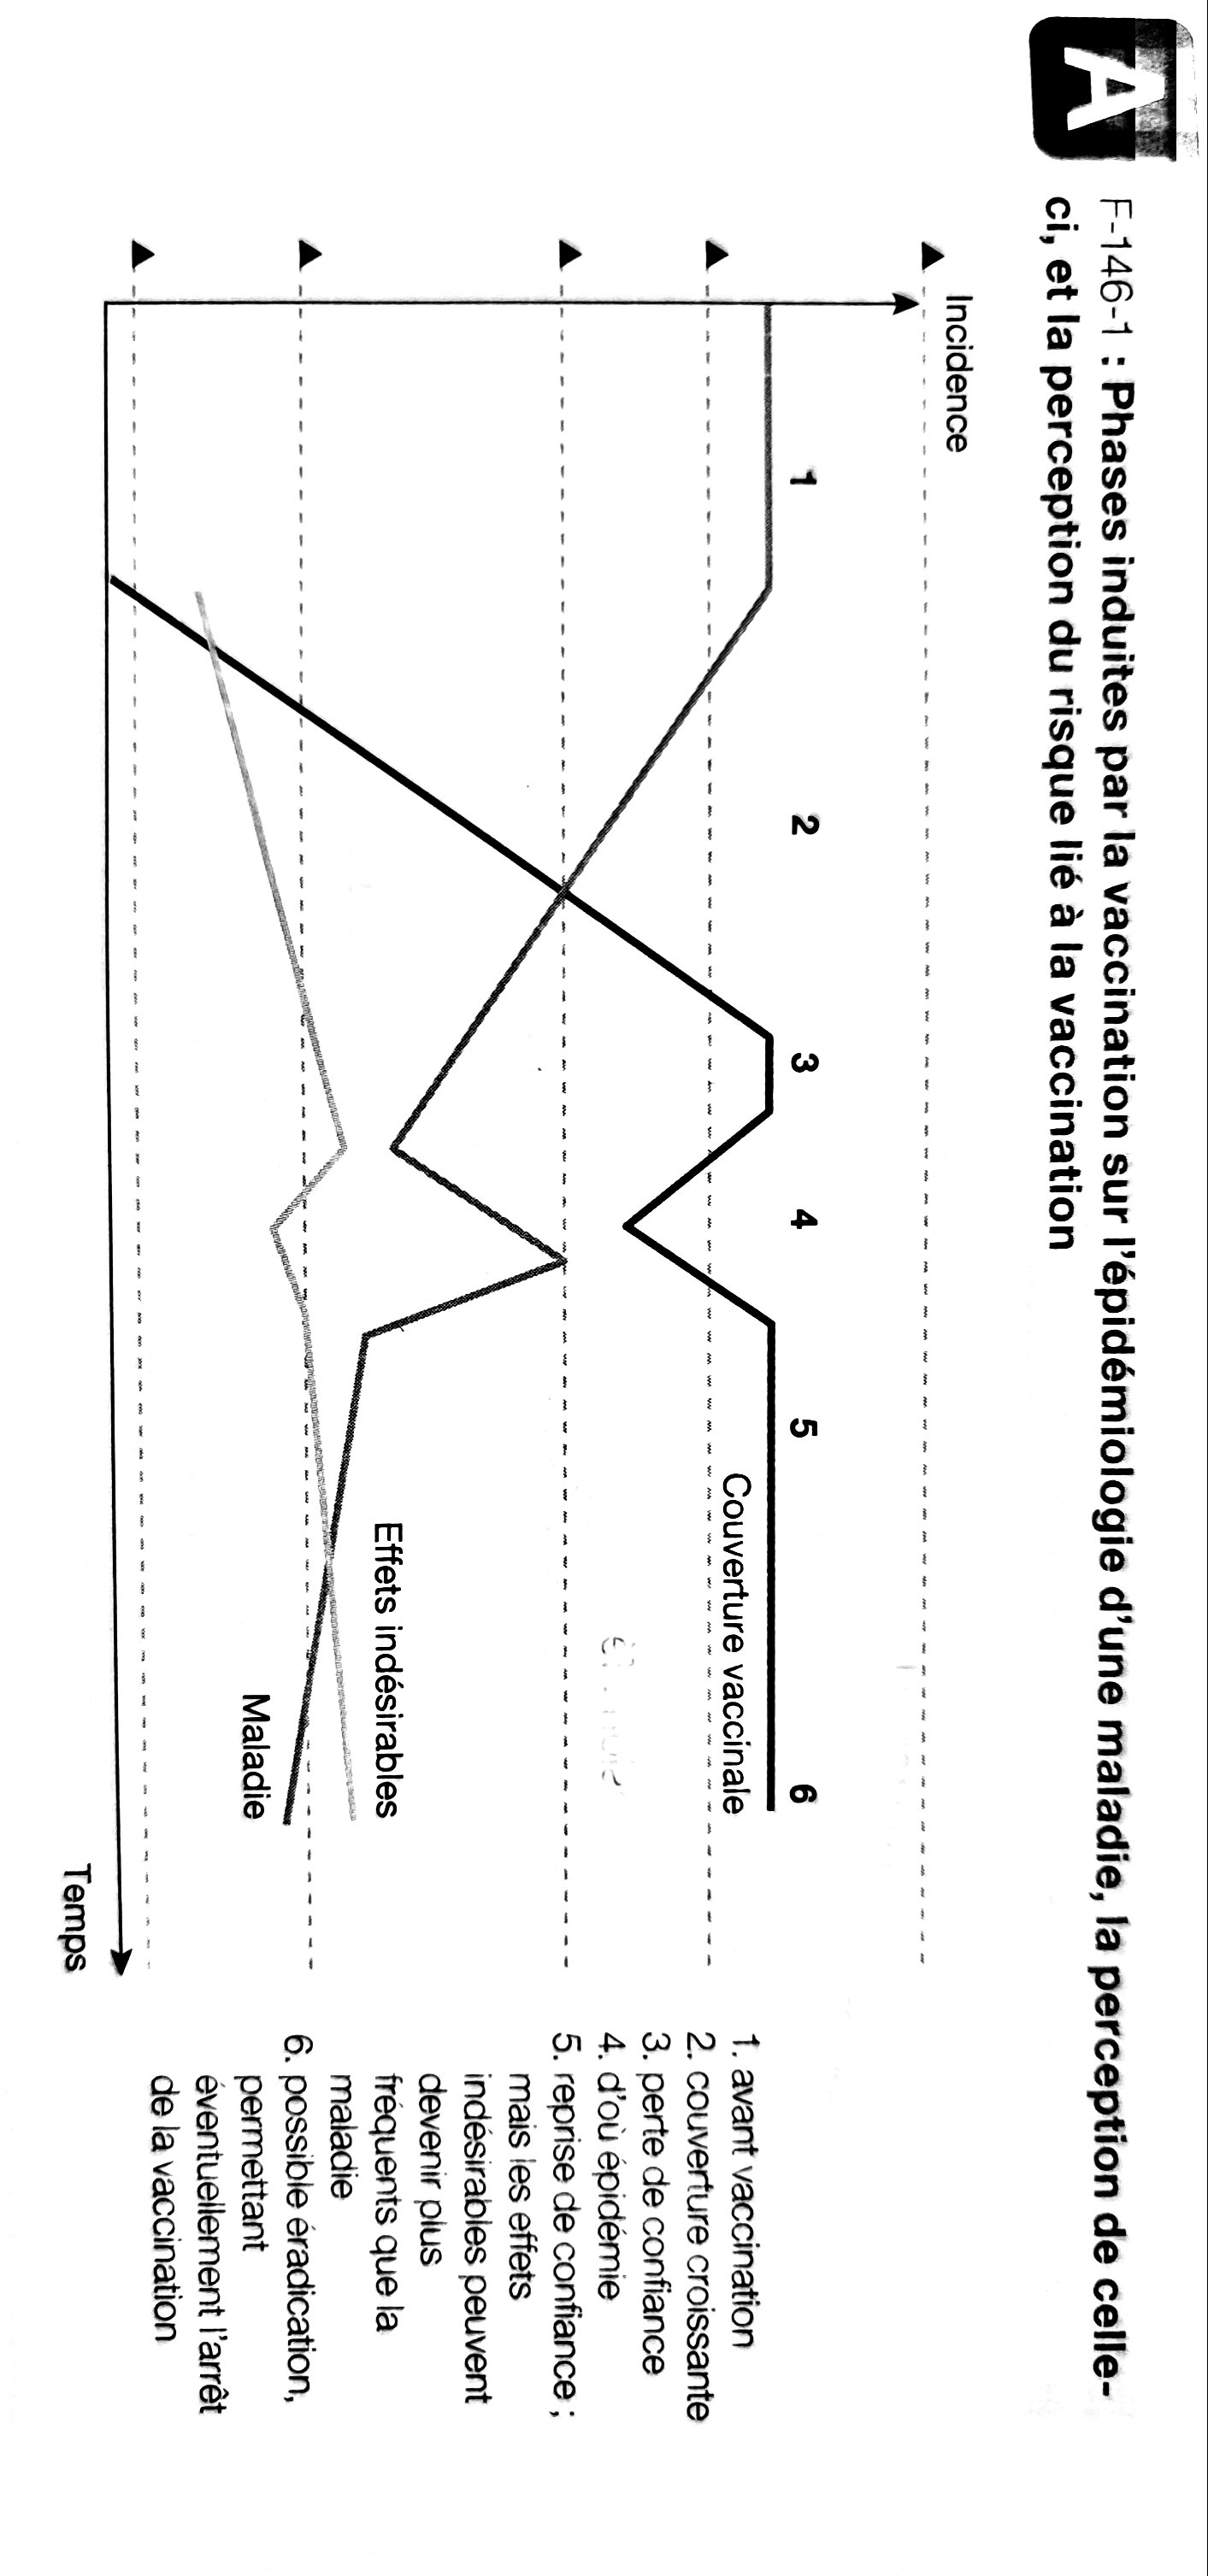
\includegraphics[width=0.4\textwidth, angle=90]{imgs/Perception.jpg} % Pilly 2021 Etudiant CMIT 1st edition
                    \caption{Common evolution of vaccine coverage \autocite{PILLYEtudiantMaladies}}
                \label{fig:perception}
            \end{figure}
            
            The right thing to consider should be the balance between benefits and risks, at several levels.
            Firstly it is an individual protection. 
            Secondly it protects the whole population thanks to herd immunity: the pathogen is less likely to be transmitted; otherwise it would be 
                an exponential growth,
                as people observed for the Covid-19 pandemic.
        
            Besides, new techniques can mean new fears for the population.
            Clearly long-term effects are unknown, however a lot of misinformation can be observed.
            People also criticized the loss of freedom, with devices like electronical vaccination records.
            Doubts cause measles outbreaks in the US for instance because too much people refused to be vaccinated.
            People are criticizing the money laboratories are making thanks to vaccines and the corresponding patents during the COVID-19 pandemic, 
                which can lead to a kind of reject of the vaccines and more specifically of the new promising methods.
            A lot of vulgarism should be realized because biotechnologies are more and more complex to understand
                and it is therefore difficult to have an informed opinion on the subject. 
            Indeed, several studies proved that it is not dangerous for health, especially for the doubts about metal adjuvants.

    \subsection{Uses and ethics}
        
        Currently, there is no real therapeutic vaccines, which would avoid the expression of the disease after the infection (it is only prophylatic).
            However promising plans are studied as presented in \ref{fig:vaccEvolution}.
            In the document, "prime" means a pathogen which has already been encountered. It can lead to what is called the "antigenic sin", 
            since the immune system is shaped with a particular response for each individual. Developing an efficient vaccine for a whole population would therefore be more difficult,
            that is the reason why therapeutic vaccines are still a challenge.

        \begin{figure}
            \centering
            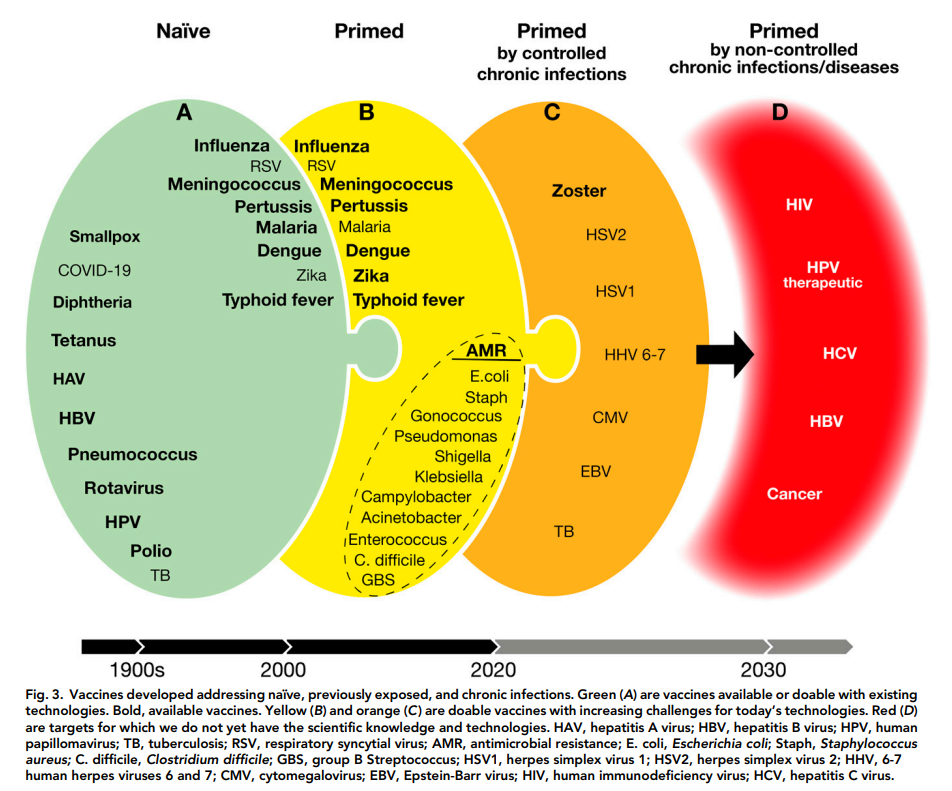
\includegraphics[width=0.75\textwidth]{imgs/vaccineEvolution.PNG}
            \caption{What to expect about vaccines? \autocite{rappuoliVaccinologyPostCOVID192021}}
            \label{fig:vaccEvolution}
        \end{figure}

        Another major aspect to consider as regards biotechnologies is the ethical one.
        As Rabelais said, "science without conscience is but the ruin of the soul".
        Now that technology gives us so many possibilites, 
        going as far as changing our genes (even if that it is clearly not the case with mRNA vaccines), what is morally acceptable? 
        Thererefore, there are the scientific abilities, the ethical aspects and the regulation, which can be very different.
        The movie \emph{Welcome to GATTACA}, directed by Andrew Nicol, offers an example of a society currently perceived as dystopic.
        More basically, the ethics of clinical trials were mainly established with the Nuremberg Code after the World War II,
            it requires consent and the absence of voluntary infection.
        
    \section{Conclusion}

        Clearly, vaccination is a miracle since the eighteenth century.
        It has led to the eradication of smallpox. Polyomyelite and diphteria are following the same path.
        According to estimations from the WHO, 50 million future deaths could be averted from 2021 to 2030.
        Thanks to medicine, biology, chemistry and computer science, 
            the recent breakthrough about mRNA vaccines, despite (or thanks to) the pandemic, allows firms to develop more quickly safer vaccines.
        However, today is a turning point to avoid people from rejecting this powerful technology by fear: government should be careful but ambitious
            as regards regulation. 
            Science is not enough: vaccine acceptance is as important as vaccine development.
            The Figure \ref{fig:agenda2} sums up the different aspects to work on in the near future and globally.

        \begin{figure}
            \centering
            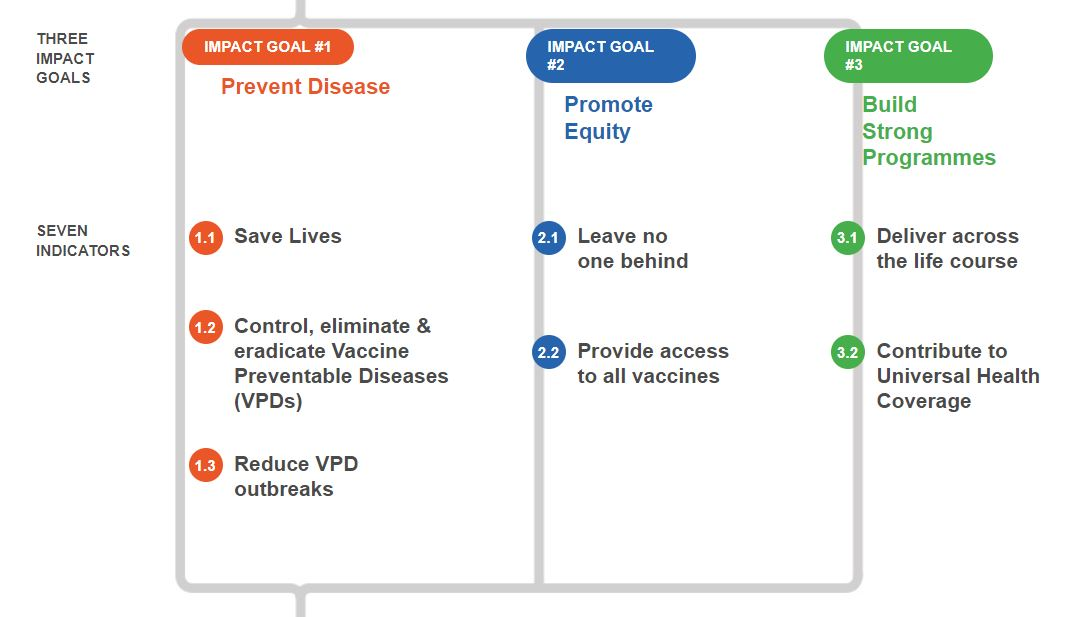
\includegraphics[width=0.75\textwidth]{imgs/Objectives.JPG}
            \caption{Immunization agenda 2030 (source WHO)}
            \label{fig:agenda2}
        \end{figure}  

    %https://biontech.de/covid-19-portal/mrna-vaccines (interesting schema)
    %https://sitn.hms.harvard.edu/flash/2015/rna-vaccines-a-novel-technology-to-prevent-and-treat-disease/
    % Bill & Melinda Gates Foundation invested $53 million in the German company, CureVac, which specializes in the development of these vaccines
    % perspective for the future as regard influenza vaccines : influenza vaccine, whereas the company CureVac claims that RNA-based vaccines could be manufactured in less than two months at a lower production cost, (harvard) + cancer vaccines

    \clearpage
    
    \nocite{*}
    \printbibliography

    \clearpage

    \appendix

    \section {Source code}
        The source code of this document is available at \url{https://github.com/florian6973/biology-report}.
        It was written using Visual Studio Code and compiled with TeX Live (Windows).

        In this repository a beamer is also available, to present this report.

        Bibliography was organized using Zotero, Better Bibtex and its browser extension.

\end{document}